\section{Ejercicio 1}

En este trabajo se abordaron los conceptos de \textit{Computational Graphs} y \textit{Back Propagation} para entrenar una red neuronal densa.
Un \textbf{grafo computacional} es una manera de representar una función matemática en el lenguaje de la teoría de grafos. En el grafo, cada nodo representa un valor de una variable o una función que combina valores. Los valores que ingresan o salen de los nodos se denominan \textbf{Tensores}.

Utilizando el concepto de \textbf{grafos computacionales} se busca implementar las funciones \textbf{Sigmoide}, \textbf{Tanh}, \textbf{ELU} y \textbf{Leaky Relu}, tomando como entrada:
$x=[2.8, -1.8]$, $W=[1.45, -0.35]$, $b=-4$. En los siguientes grafos, los valores en color negro indican los resultados del proceso hacia adelante (\textit{forward}) mientras que en rojo se colocan los resultados del \textit{Backpropagation} recordando que el valor del gradiente a la salida del grafo es 1.

\subsection{Sigmoide}

\begin{equation}
    f(x)=\frac{1}{1+e^{-x}};\ \ f'(x)=\sigma(x)(1-\sigma(x))
\end{equation}
\vspace{1cm}
\hspace{1.5cm}
% first of all, we define our grid
\begin{VCPicture}{(0,-3)(6,3)}

% and then we create the states
\ChgEdgeLabelScale{0.5}
\ChgEdgeLabelSep{.5}
\LargeState
\VSState{(-1.5,1.5)}{S1}
\VSState{(-1.5,0)}{S2}
\VSState{(-1.5,-1.5)}{S3}
\VSState{(-1.5,-3)}{S4}
\VSState{(-1.5,-4.5)}{S5}

\State[w_0]{(0,1.5)}{STATEA}
\State[x_0]{(0,0)}{STATEB}
\State[w_1]{(0,-1.5)}{STATEC}
\State[x_1]{(0,-3)}{STATED}
\State[b]{(2,-4.5)}{STATEE}

\State[\times]{(2,0.75)}{STATEF}
\State[\times]{(2,-2.25)}{STATEG}

\State[+]{(4.5,-.75)}{STATEH}


\StateVar[\times(-1)]{(7,-.75)}{STATEI}

\State[\exp]{(9.5,-.75)}{STATEJ}
\State[+1]{(11.5,-.75)}{STATEK}
\State[1/x]{(13.5,-.75)}{STATEL}
\VSState{(15.5,-.75)}{ENDSTATE}
% now, transition time

% straight lines
\EdgeR{S1}{STATEA}{1.45}
\EdgeR{S2}{STATEB}{2.8}
\EdgeR{S3}{STATEC}{-0.35}
\EdgeR{S4}{STATED}{-1.8}
\EdgeR{S5}{STATEE}{-4}

\LArcR{STATEA}{STATEF}{}
\LArcL{STATEB}{STATEF}{}
\LArcR{STATEC}{STATEG}{}
\LArcL{STATED}{STATEG}{}

\ArcR{STATEF}{STATEH}{4.060}
\ArcR{STATEG}{STATEH}{0.630}
\LArcR{STATEE}{STATEH}{}

\LArcL{STATEH}{STATEI}{0.690}
\LArcL{STATEI}{STATEJ}{-0.690}
\LArcL{STATEJ}{STATEK}{1.994}
\LArcL{STATEK}{STATEL}{2.994}

\EdgeR{STATEL}{ENDSTATE}{0.334}

\ChgEdgeLineColor{red}
\ChgEdgeLineStyle{dashed}
\ChgEdgeLabelColor{red}

\LArcL{STATEL}{STATEK}{-0.112}
\LArcL{STATEK}{STATEJ}{-0.112}
\LArcL{STATEJ}{STATEI}{-0.056}
\LArcL{STATEI}{STATEH}{0.056}

\ArcR{STATEH}{STATEF}{0.056}
\ArcR{STATEH}{STATEG}{0.056}
\ArcL{STATEH}{STATEE}{0.056}

\LArcR{STATEF}{STATEA}{0.157}
\LArcL{STATEF}{STATEB}{0.081}
\LArcR{STATEG}{STATEC}{-0.101}
\LArcL{STATEG}{STATED}{-0.020}


% loops
% \LoopN{STATEA}{0.1}
% \LoopW{STATEB}{0.4}
% \LoopE{STATED}{0.6}

\end{VCPicture}
\newline

\begin{figure}[H]
    \centering
    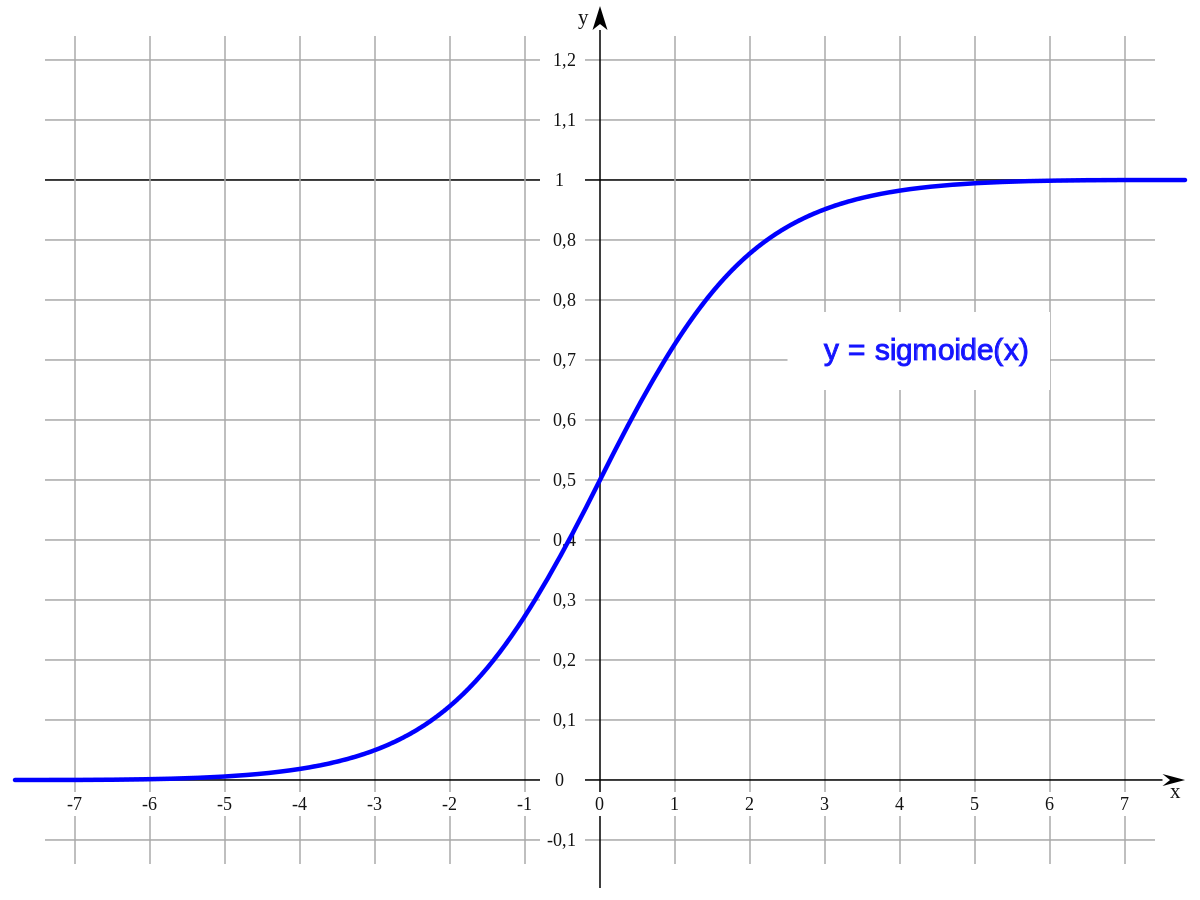
\includegraphics[height=2in]{image/sigmoide}
    \caption{Función Sigmoide ($\sigma(x))$}
    \label{fig:my_label}
\end{figure}


\subsection{Tanh}

\begin{equation}
    f(x)=tanh(x)=\frac{e^{-x}-1}{e^{-x}+1}; \ \ f'(x)=1-tanh^2(x)
\end{equation}
\vspace{1cm}
\hspace{1.5cm}
% first of all, we define our grid
\begin{VCPicture}{(0,-3)(6,3)}

% and then we create the states
\ChgEdgeLabelScale{0.5}
% \ChgEdgeLabelSep{}
\LargeState
\VSState{(-1.5,1.5)}{S1}
\VSState{(-1.5,0)}{S2}
\VSState{(-1.5,-1.5)}{S3}
\VSState{(-1.5,-3)}{S4}
\VSState{(-1.5,-4.5)}{S5}

\State[w_0]{(0,1.5)}{STATEA}
\State[x_0]{(0,0)}{STATEB}
\State[w_1]{(0,-1.5)}{STATEC}
\State[x_1]{(0,-3)}{STATED}
\State[b]{(2,-4.5)}{STATEE}

\State[\times]{(2,0.75)}{STATEF}
\State[\times]{(2,-2.25)}{STATEG}

\State[+]{(4.5,-.75)}{STATEH}


\StateVar[\times(2)]{(6.5,-.75)}{STATEI}

\State[\exp]{(9,-.75)}{STATEJ}

\State[-1]{(11,1)}{STATEK}
\State[+1]{(11,-2.5)}{STATEL}

\State[\frac{a}{b}]{(13,-.75)}{STATEM}

\VSState{(15,-.75)}{ENDSTATE}
% now, transition time

% straight lines
\EdgeR{S1}{STATEA}{1.45}
\EdgeR{S2}{STATEB}{2.8}
\EdgeR{S3}{STATEC}{-0.35}
\EdgeR{S4}{STATED}{-1.8}
\EdgeR{S5}{STATEE}{-4}

\LArcR{STATEA}{STATEF}{}
\LArcL{STATEB}{STATEF}{}
\LArcR{STATEC}{STATEG}{}
\LArcL{STATED}{STATEG}{}

\ArcR{STATEF}{STATEH}{4.060}
\ArcR{STATEG}{STATEH}{0.630}
\LArcR{STATEE}{STATEH}{}

\LArcL{STATEH}{STATEI}{0.690}
\LArcL{STATEI}{STATEJ}{1.38}
% \ArcL{A}{B}{\IOL{2}{0}}
\LArcL{STATEJ}{STATEK}{3.975}
\LArcR{STATEJ}{STATEL}{3.975}

\LArcL{STATEK}{STATEM}{2.975}
\LArcR{STATEL}{STATEM}{4.975}

\EdgeR{STATEM}{ENDSTATE}{0.598}

\ChgEdgeLineColor{red}
\ChgEdgeLineStyle{dashed}
\ChgEdgeLabelColor{red}

\ArcR{STATEM}{STATEL}{-0.120}
\ArcL{STATEM}{STATEK}{0.201}

\ArcR{STATEL}{STATEJ}{-0.120}
\ArcL{STATEK}{STATEJ}{0.201}

\LArcL{STATEJ}{STATEI}{0.322}
\LArcL{STATEI}{STATEH}{0.644}

\ArcR{STATEH}{STATEF}{0.644}
\ArcR{STATEH}{STATEG}{0.644}
\ArcL{STATEH}{STATEE}{0.644}

\LArcR{STATEF}{STATEA}{1.803}
\LArcL{STATEF}{STATEB}{0.934}
\LArcR{STATEG}{STATEC}{-1.159}
\LArcL{STATEG}{STATED}{-0.225}



% loops
% \LoopN{STATEA}{0.1}
% \LoopW{STATEB}{0.4}
% \LoopE{STATED}{0.6}

\end{VCPicture}
\newline

\begin{figure}[H]
    \centering
    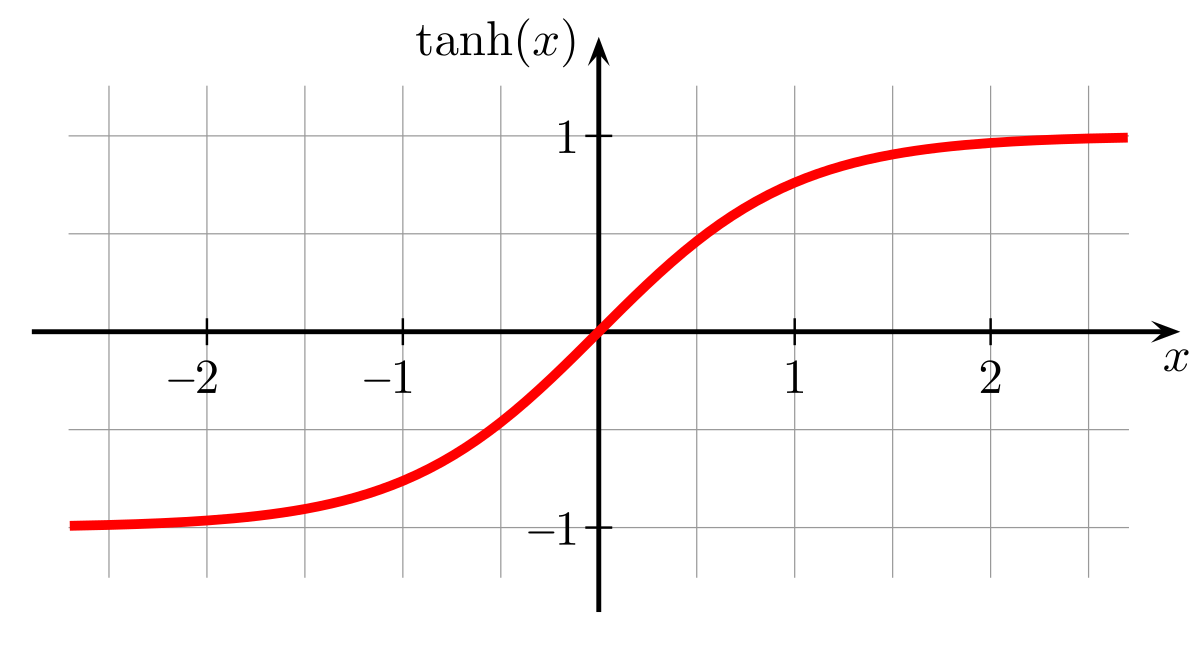
\includegraphics[height=2in]{image/tanh}
    \caption{Función Tangente Hiperbólica ($tanh(x)$)}
    \label{fig:my_label}
\end{figure}

\subsection{ELU}

\[   
f(a,b) = 
     \begin{cases}
        \text{x} & x \geq 0 \\
       \text{$\alpha (\exp(x)-1)$} & x < 0 \\
     \end{cases}
\]
\vspace{1cm}
\hspace{5.5cm}
% first of all, we define our grid
\begin{VCPicture}{(0,-3)(6,3)}

% and then we create the states
\ChgEdgeLabelScale{0.5}
\ChgEdgeLabelSep{.5}
\LargeState
\VSState{(-1.5,1.5)}{S1}
\VSState{(-1.5,0)}{S2}
\VSState{(-1.5,-1.5)}{S3}
\VSState{(-1.5,-3)}{S4}
\VSState{(-1.5,-4.5)}{S5}

\State[w_0]{(0,1.5)}{STATEA}
\State[x_0]{(0,0)}{STATEB}
\State[w_1]{(0,-1.5)}{STATEC}
\State[x_1]{(0,-3)}{STATED}
\State[b]{(2,-4.5)}{STATEE}

\State[\times]{(2,0.75)}{STATEF}
\State[\times]{(2,-2.25)}{STATEG}

\State[+]{(4.5,-.75)}{STATEH}


% \StateVar[\times(-1)]{(7,-.75)}{STATEI}

% \State[\exp]{(9.5,-.75)}{STATEJ}
% \State[+1]{(11.5,-.75)}{STATEK}
% \State[1/x]{(13.5,-.75)}{STATEL}
\VSState{(7,-.75)}{ENDSTATE}
% now, transition time

% straight lines
\EdgeR{S1}{STATEA}{1.45}
\EdgeR{S2}{STATEB}{2.8}
\EdgeR{S3}{STATEC}{-0.35}
\EdgeR{S4}{STATED}{-1.8}
\EdgeR{S5}{STATEE}{-4}

\LArcR{STATEA}{STATEF}{}
\LArcL{STATEB}{STATEF}{}
\LArcR{STATEC}{STATEG}{}
\LArcL{STATED}{STATEG}{}

\ArcR{STATEF}{STATEH}{4.060}
\ArcR{STATEG}{STATEH}{0.630}
\LArcR{STATEE}{STATEH}{}

% \LArcL{STATEH}{STATEI}{0.690}
% \LArcL{STATEI}{STATEJ}{-0.690}
% \LArcL{STATEJ}{STATEK}{1.994}
% \LArcL{STATEK}{STATEL}{2.994}

\EdgeR{STATEH}{ENDSTATE}{0.0.690}

\ChgEdgeLineColor{red}
\ChgEdgeLineStyle{dashed}
\ChgEdgeLabelColor{red}

% \LArcL{STATEL}{STATEK}{-0.112}
% \LArcL{STATEK}{STATEJ}{-0.112}
% \LArcL{STATEJ}{STATEI}{-0.056}
% \LArcL{STATEI}{STATEH}{0.056}

\ArcR{STATEH}{STATEF}{1}
\ArcR{STATEH}{STATEG}{1}
\ArcL{STATEH}{STATEE}{1}

\LArcR{STATEF}{STATEA}{2.8}
\LArcL{STATEF}{STATEB}{1.450}
\LArcR{STATEG}{STATEC}{-1.800}
\LArcL{STATEG}{STATED}{-0.350}


% loops
% \LoopN{STATEA}{0.1}
% \LoopW{STATEB}{0.4}
% \LoopE{STATED}{0.6}

\end{VCPicture}
\newline
\vspace{1cm}
\hspace{1.5cm}
% first of all, we define our grid
\begin{VCPicture}{(0,-3)(6,3)}

% and then we create the states
\ChgEdgeLabelScale{0.5}
\ChgEdgeLabelSep{.5}
\LargeState
\VSState{(-1.5,1.5)}{S1}
\VSState{(-1.5,0)}{S2}
\VSState{(-1.5,-1.5)}{S3}
\VSState{(-1.5,-3)}{S4}
\VSState{(-1.5,-4.5)}{S5}

\State[w_0]{(0,1.5)}{STATEA}
\State[x_0]{(0,0)}{STATEB}
\State[w_1]{(0,-1.5)}{STATEC}
\State[x_1]{(0,-3)}{STATED}
\State[b]{(2,-4.5)}{STATEE}

\State[\times]{(2,0.75)}{STATEF}
\State[\times]{(2,-2.25)}{STATEG}

\State[+]{(4.5,-.75)}{STATEH}


\State[\exp]{(7,-.75)}{STATEI}
\State[-1]{(9.5,-.75)}{STATEJ}
\StateVar[\times\alpha]{(12,-.75)}{STATEK}
\VSState{(14.5,-.75)}{ENDSTATE}
% now, transition time

% straight lines
\EdgeR{S1}{STATEA}{1.45}
\EdgeR{S2}{STATEB}{2.8}
\EdgeR{S3}{STATEC}{-0.35}
\EdgeR{S4}{STATED}{-1.8}
\EdgeR{S5}{STATEE}{-4}

\LArcR{STATEA}{STATEF}{}
\LArcL{STATEB}{STATEF}{}
\LArcR{STATEC}{STATEG}{}
\LArcL{STATED}{STATEG}{}

\ArcR{STATEF}{STATEH}{4.060}
\ArcR{STATEG}{STATEH}{0.630}
\LArcR{STATEE}{STATEH}{}

\LArcL{STATEH}{STATEI}{0.690}

\LArcL{STATEI}{STATEJ}{1.994}
\LArcL{STATEJ}{STATEK}{0.994}
\EdgeR{STATEK}{ENDSTATE}{\alpha 0.994}

% \EdgeR{STATEK}{ENDSTATE}{\alpha 0.994}

\ChgEdgeLineColor{red}
\ChgEdgeLineStyle{dashed}
\ChgEdgeLabelColor{red}

% \LArcL{STATEL}{STATEK}{-0.112}
\LArcL{STATEK}{STATEJ}{\alpha}
\LArcL{STATEJ}{STATEI}{\alpha}
\LArcL{STATEI}{STATEH}{\alpha 1.994}

\ArcR{STATEH}{STATEF}{\alpha 1.994}
\ArcR{STATEH}{STATEG}{\alpha 1.994}
\ArcL{STATEH}{STATEE}{\alpha 1.994}

\LArcR{STATEF}{STATEA}{\alpha 5.583}
\LArcL{STATEF}{STATEB}{\alpha 2.891}
\LArcR{STATEG}{STATEC}{-\alpha 3.589}
\LArcL{STATEG}{STATED}{-\alpha 0.698}


% loops
% \LoopN{STATEA}{0.1}
% \LoopW{STATEB}{0.4}
% \LoopE{STATED}{0.6}

\end{VCPicture}
\newline
\newline

\begin{figure}[H]
    \centering
    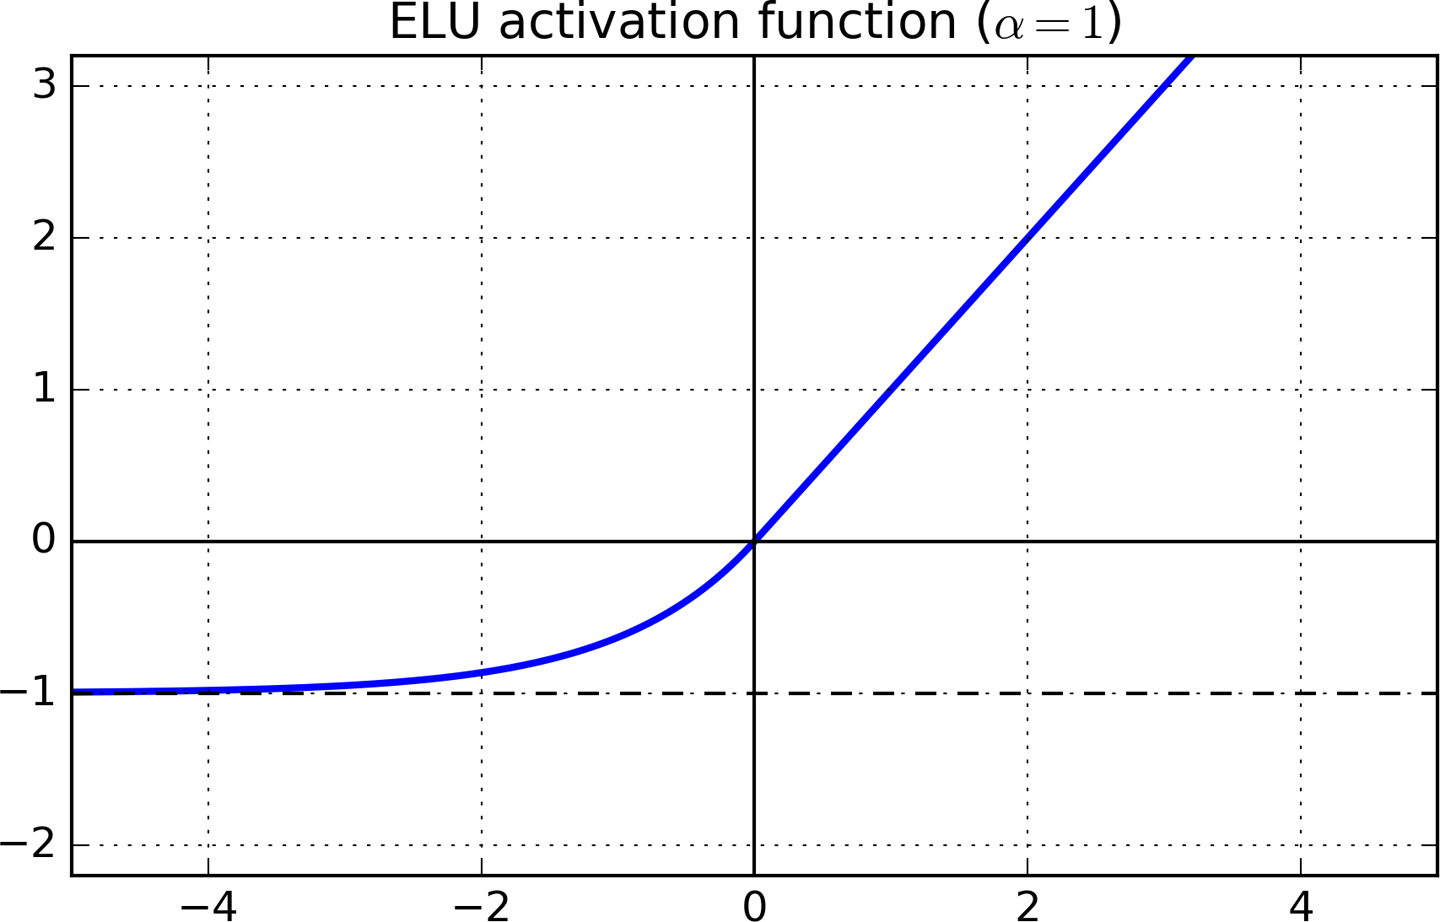
\includegraphics[height=2in]{image/ELU}
    \caption{Función de activación ELU}
    \label{fig:my_label}
\end{figure}



\subsection{Leaky Relu}

\begin{equation}
    f(x)=LeakyRelu(x)=max(0.1x, x)
\end{equation}
\vspace{1cm}
\hspace{3.5cm}
% first of all, we define our grid
\begin{VCPicture}{(0,-3)(6,3)}

% and then we create the states
\ChgEdgeLabelScale{0.5}
% \ChgEdgeLabelSep{}
\LargeState
\VSState{(-1.5,1.5)}{S1}
\VSState{(-1.5,0)}{S2}
\VSState{(-1.5,-1.5)}{S3}
\VSState{(-1.5,-3)}{S4}
\VSState{(-1.5,-4.5)}{S5}

\State[w_0]{(0,1.5)}{STATEA}
\State[x_0]{(0,0)}{STATEB}
\State[w_1]{(0,-1.5)}{STATEC}
\State[x_1]{(0,-3)}{STATED}
\State[b]{(2,-4.5)}{STATEE}

\State[\times]{(2,0.75)}{STATEF}
\State[\times]{(2,-2.25)}{STATEG}

\State[+]{(4.5,-.75)}{STATEH}


\StateVar[\times(0.1)]{(6.5,1)}{STATEI}
\StateVar[\times 1]{(6.5,-2.5)}{STATEJ}
% \State[\exp]{(9,-.75)}{STATEJ}

\StateVar[MAX]{(9,-.75)}{STATEK}
% \State[+1]{(11,-2.5)}{STATEL}

% \State[\frac{a}{b}]{(13,-.75)}{STATEM}

\VSState{(11,-.75)}{ENDSTATE}
% now, transition time

% straight lines
\EdgeR{S1}{STATEA}{1.45}
\EdgeR{S2}{STATEB}{2.8}
\EdgeR{S3}{STATEC}{-0.35}
\EdgeR{S4}{STATED}{-1.8}
\EdgeR{S5}{STATEE}{-4}

\LArcR{STATEA}{STATEF}{}
\LArcL{STATEB}{STATEF}{}
\LArcR{STATEC}{STATEG}{}
\LArcL{STATED}{STATEG}{}

\ArcR{STATEF}{STATEH}{4.060}
\ArcR{STATEG}{STATEH}{0.630}
\LArcR{STATEE}{STATEH}{}

\LArcL{STATEH}{STATEI}{0.690}
\LArcR{STATEH}{STATEJ}{0.690}
% \ArcL{A}{B}{\IOL{2}{0}}
\LArcL{STATEI}{STATEK}{0.069}
\LArcR{STATEJ}{STATEK}{0.690}

% \LArcL{STATEK}{STATEM}{2.975}
% \LArcR{STATEL}{STATEM}{4.975}

\EdgeR{STATEK}{ENDSTATE}{0.690}

\ChgEdgeLineColor{red}
\ChgEdgeLineStyle{dashed}
\ChgEdgeLabelColor{red}

% \ArcR{STATEM}{STATEL}{-0.120}
% \ArcL{STATEM}{STATEK}{0.201}

% \ArcR{STATEL}{STATEJ}{-0.120}
\ArcL{STATEK}{STATEI}{0}
\ArcR{STATEK}{STATEJ}{1}

\LArcR{STATEJ}{STATEH}{1}
\LArcL{STATEI}{STATEH}{0}

\ArcR{STATEH}{STATEF}{1}
\ArcR{STATEH}{STATEG}{1}
\ArcL{STATEH}{STATEE}{1}

\LArcR{STATEF}{STATEA}{2.8}
\LArcL{STATEF}{STATEB}{1.45}
\LArcR{STATEG}{STATEC}{-1.8}
\LArcL{STATEG}{STATED}{-0.35}



% loops
% \LoopN{STATEA}{0.1}
% \LoopW{STATEB}{0.4}
% \LoopE{STATED}{0.6}

\end{VCPicture}
\newline
\newline
\newline

\begin{figure}[H]
    \centering
    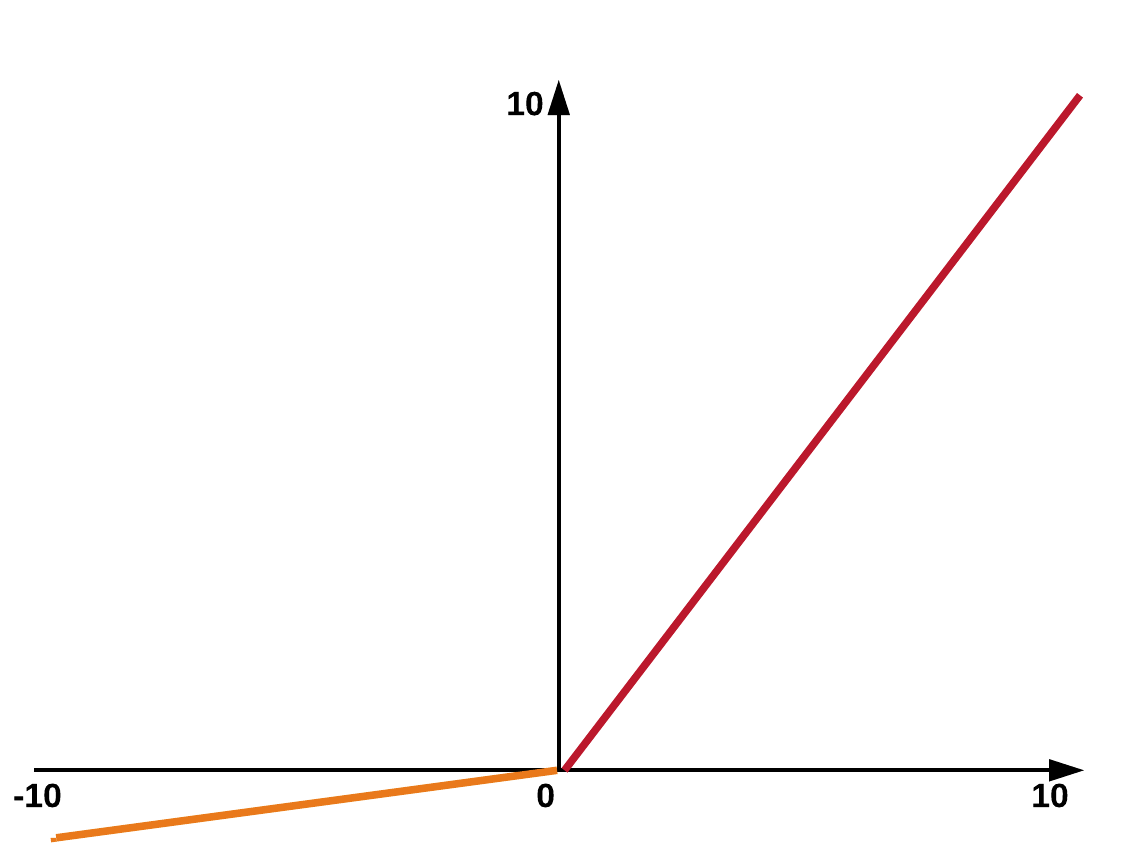
\includegraphics[height=2in]{image/relu}
    \caption{Función Leaky Relu}
    \label{fig:my_label}
\end{figure}

La elección de la función de activación para una capa de una red neuronal depende de los valores de salida que se requieren y de las propiedades de la función de activación utilizada. Por ejemplo, si se trabajan con probabilidades, podría pensarse en usar la función de activación \textbf{Sigmoide} dado que esta función tiene la salida acotada entre 0 y 1, si se trabaja con valores positivos se pensaría en usar la función \textbf{Relu} que anula los valores negativos y para valores generales, se pensaría en usar la función de activación \textbf{Lineal}.

En esquemas con más de una capa, uno preferiría usar la función \textbf{Leaky Relu} en lugar de la \textbf{Relu}, la cual permite ser más permisivo al no anular completamente ciertas neuronas y por el mismo motivo, se prefiere usar la función \textbf{tanh} en lugar de la \textbf{Sigmoide}.


